\documentclass[parskip,
							 oneside,
% 							 longdoc,
							 11pt,
							 noheadingspace,
							 accentcolor=tud1d,
							 bigchapter,
							 %draft,
							 enabledeprecatedfontcommands,
							 colorback]{tudreport}


%% Spracheinstellungen
\usepackage[ngerman]{babel}
%\usepackage[applemac]{inputenc} % Input-Encodung: applemac fuer Mac
%\IfFileExists{latin1.sty}{\usepackage{latin1}}{\usepackage{isolatin1}}
%\usepackage[latin1]{inputenc}
%\usepackage[T1]{fontenc}
\usepackage[ansinew]{inputenc}  % Input-Encodung: ansinew fuer Windows
\usepackage{microtype} % optischer Randausgleich bei pdflatex mit Zeichendehnung

%% Grafikeinstellungen
\usepackage{float} % u.a. genaue Plazierung von Gleitobjekten mit H
%\usepackage[latin1]{inputenc}


%% Tabelleneinstellungen
\usepackage{booktabs}
\usepackage{multirow}
\usepackage{longtable}
\usepackage{tabularx}

%% State Chart
\usepackage{pgf}
\usepackage{tikz}
\usetikzlibrary{arrows,automata}

%% Mathematik
\usepackage{amsmath}
\usepackage{nicefrac}
\usepackage{icomma}

%% sonstige Einstellungen
\usepackage{paralist}% erweiterte Listenumgebung (z.B. compactitem)
\usepackage{textcomp} % verschiedene Symbole
\usepackage[nottoc, numbib]{tocbibind}
\usepackage{hyperref}
\renewcommand\plparsep{1ex}
\usepackage{enumerate}


\title{\textbf{Hardware Design Lab}}
\subtitle{Report Group 6}
\subsubtitle{Lukas Boland, Sven Str\"oher, Ana Carolina Ferreira, Julian K\"auser \\
Supervisor: Sarath Kundumattathil Mohanan, M.Sc.\\
			 Begin: 07/31/2017 \textbar\ Submission: 08/16/2017\\
			 Institute of Computer Engineering \hfill\textbar\hfill Integrated Electronic Systems Lab\hfill\textbar\hfill Prof.\,Dr.-Ing.\, Klaus Hofmann}
\setinstitutionlogo{images/logo.png}
% \institution{Institut f\"ur Datentechnik\hfill\textbar\hfill Fachgebiet Rechnersysteme\hfill\textbar\hfill Prof.\,Dr.-Ing.\, Hans Eveking}
%\settitlepicture{images/spartan}
\begin{document}

%% Titel %%%%%%%%%%%%%%%%%%%%%%%%%%%%%%%%%%%%%%%%%%%%%%%%%%%%%%%%%%%%%%%%%%
\maketitle
\cleardoublepage

%% Vorgeplnkel %%%%%%%%%%%%%%%%%%%%%%%%%%%%%%%%%%%%%%%%%%%%%%%%%%%%%%%%%%%%%%
\pagestyle{empty}
%\pagenumbering{roman}


%% Hauptteil %%%%%%%%%%%%%%%%%%%%%%%%%%%%%%%%%%%%%%%%%%%%%%%%%%%%%%%%%%%%%%%
\pagestyle{headings}
\pagenumbering{arabic}
\chapter{Introduction}
\label{cha:introduction}

This semester's task in the HDL Lab is to design a general purpose processor implementing the ARM-Thumb architecture, and synthesize it with the Synopsis Design Compiler for the TSMC 45nm Standard Cell library. Further requirements are the RTL design with Verilog, the introduction of a pipelined design, the use of a given 1-Port memory and the implementation of the full instruction set. All these requirements have been met with our design, as pointed out in this report.\\ The paper is structured as following. At first, the different tasks are reviewed, and their distribution among the team members is outlined. An overview on our apporach is given. Then, the processor design and its submodules are reviewed. Furthermore, the RTL verification steps are shown. After a section on the synthesis process, the gate level verification results are shown. Finally, an evaluation of our design with regards to the task is done.

\section{Tasks and Work Distribution}
\label{sec:tasksandworkdistribution}

The task of the HDL Lab can be split into two major parts: micro-architecture design and RTL coding, and standard cell synthesis. Since the second part requires results of the first one, we started with the rtl design. 

First, the necessary submodules in the processor were agreed upon, and each team member was assigned one or more modules to work on. Creating and running a testbench for each designed module must always be performed in time with the module itself, so we assigned that task to everyone designing a module. Along with the module design, requirements regarding the Thumb-architecture had to be checked and built in. 

In the next step on the RTL level, finished and tested modules were integrated to verify their function. If necessary, a step back to the RTL design was taken in order to fix malfunctions in single modules or to adapt them to changing requirements (e.g. changing communication between modules, new necessary signals).

The second major part, standard cell synthesis, was performed from the point where some modules were finished with the RTL design. Of course, for every change in the rtl design, the synthesis had to be re-done. With regard to the synthesis results for every module, some minor adaptions in the Verilog code had to be done to guarantee the synthesizeability.

While the synthesis processes could only be started three days into the lab, they lasted until the final day. The RTL design also lasted until the end, since we tried to improve the design as far as possible. The approximate work distribution among the team members is shown below.

\begin{itemize}
\item \textbf{Lukas Boland:} RTL design (decoder) and RTL top level verification/intergration
\item \textbf{Sven Str\"oher:} RTL design (ALU, stack, fetch), synthesis, gate level verification
\item \textbf{Ana Carolina Ferreira:} RTL design (ALU, fetch, controller), synthesis, gate level verification
\item \textbf{Julian K\"auser:} RTL design (memory interface, register file, controller), short report
\end{itemize}




\chapter{Implementation}
\label{cha:implementation}

In this chapter, the designed micro-architecture is presented. Achievements from verification (both RTL and gate level) are shown. Additionally, a view on the synthesis process and results is taken.

Our design implements the Thumb architecture almost completely. It is capable of executing all instructions except \texttt{CBZ} and \texttt{CBNZ}, and all instruction related to \texttt{HINT} and \texttt{STATE CHANGE} (the last two types are explicitly not required and at least \texttt{STATE CHANGE} cannot be implemented without an ARM-capable micro-architecture). We focused on implementing all instructions, since we interpreted this as a primary objective from the lab manual. With these instructions, our processor is capable of executing both the \texttt{count32} and the \texttt{memcp46} benchmark applications.

\section{Design}
\label{sec:design}
Our design is built of relatively large submodules, so that not many additional elements are necessary in the top module. The structure can be seen in Fig. \ref{fig:processoroverview}. The main modules are the instruction decoder, the register file, the ALU, the memory interface and the instruction fetch module. These modules are described in detail in the following sections.

\begin{figure}[ht]
\centering
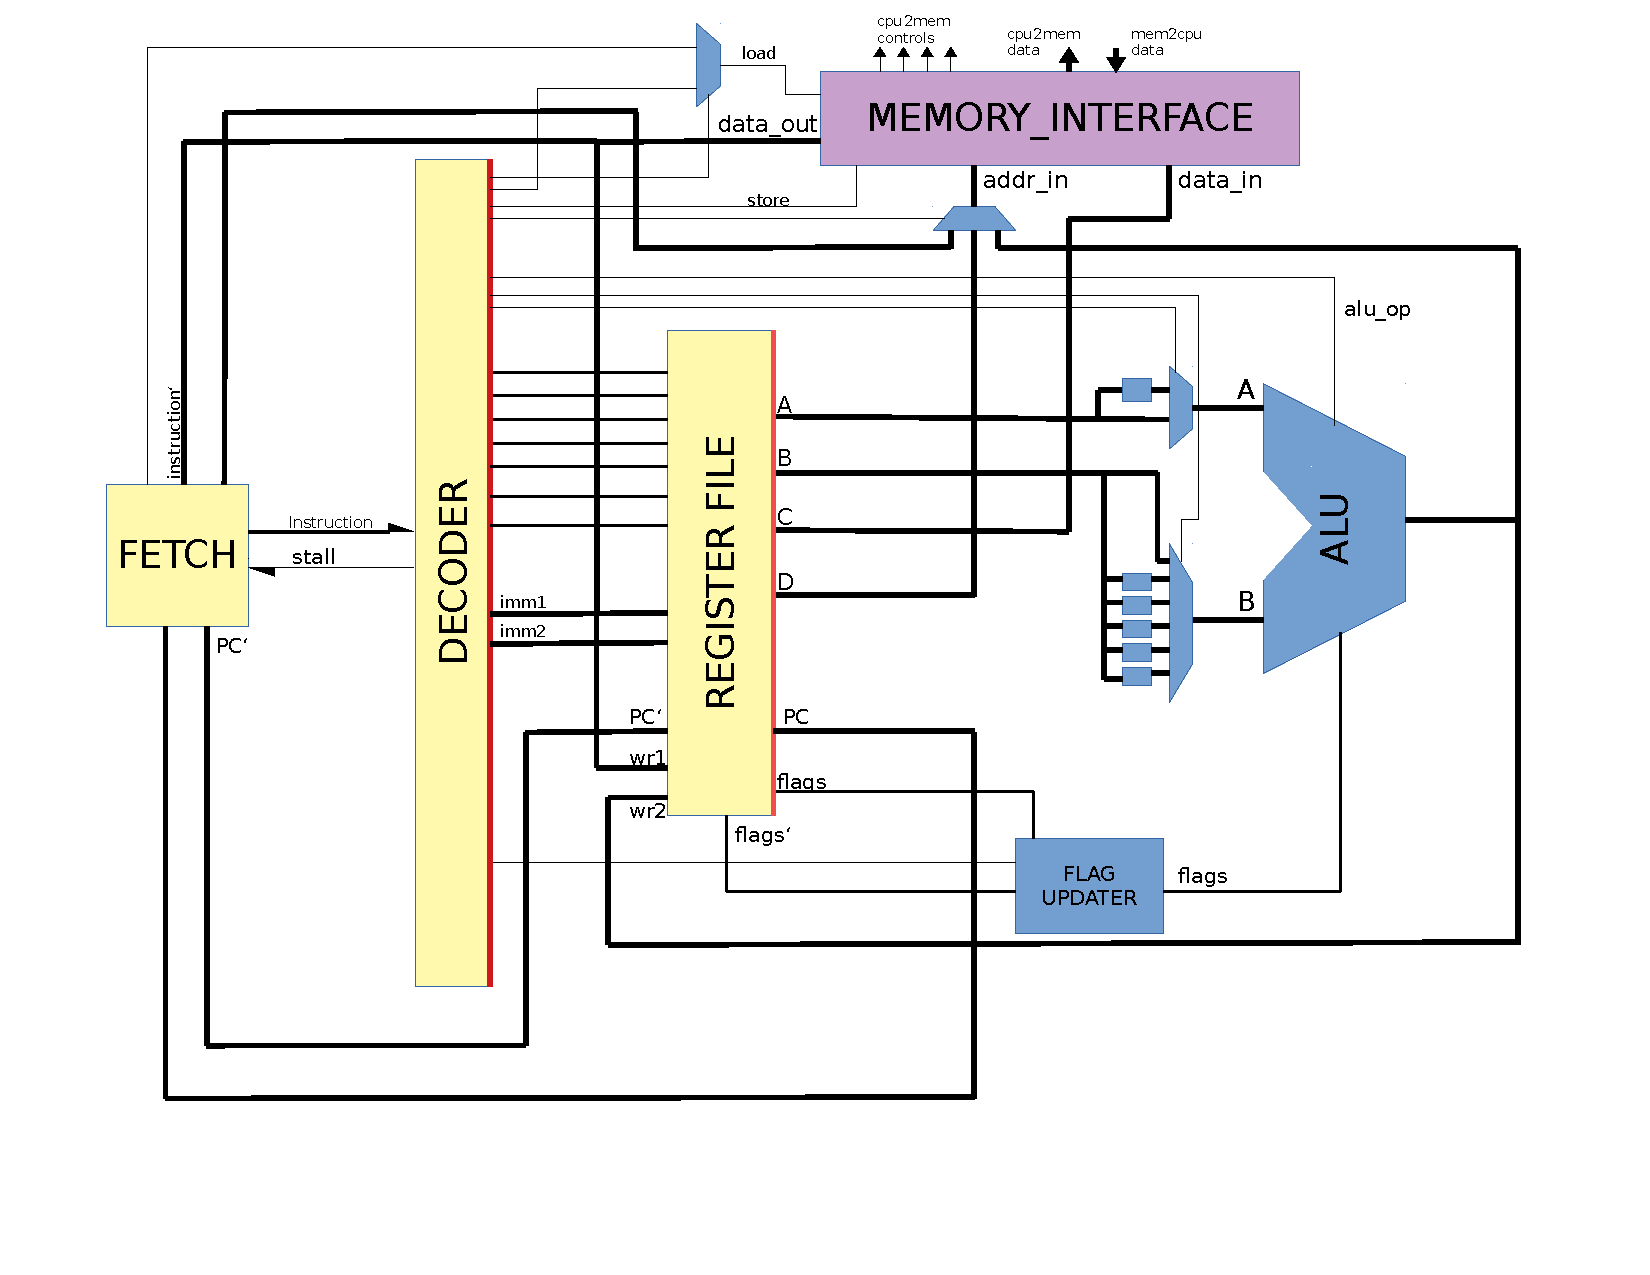
\includegraphics[scale=0.65]{images/processorOverview.pdf}
\caption{The block structure of the processor design. Register stages are marked red.}
\label{fig:processoroverview}
\end{figure}

In the block structure, the modules are connected with several connections, but only the address and load inputs for the memory are busses with more than one input. All other connections can only be driven by one module, which simplifies the overall structure. 

\subsection{Processor Control}
\label{subsec:processorcontrol}
The control of the execution and memory access is performed by a state machine in the decoder module. Initially, a dedicated controller for the memory access and pipeline stalls was planned; while integrating and testing the decoder, the function of the controller was integrated into the decoder. It yet had many control functions in order to perform multi-cycle instruction like \texttt{MULTI-PUSH/-POP}.

Almost all control signals are outputs of the decoder. These include the ALU opcode, register selects, the flag updates and memory access signals. As the memory access must be arbitrated, the instruction fetch controls the multiplexors assigning the read request and address signals from itself and the decoder module. When the current instruction accesses the memory, a stall signal to the instruction fetch can be set by the decoder. On the other hand, the instruction fetch may stall the decoder (which then stalls the rest of the processor) if the next instruction is not loaded yet. With this mechanisms, we tried to keep the control of the processor as simple as possible.

\subsection{Pipeline Stages}
\label{subsec:pipelinestages}

Our processor is comprised of two pipeline stages. One stage includes the instruction fetch and decoder, the other one does the execution and writeback tasks. These two stages have been chosen because of the structure of the benchmark applications and the 1-port memory. The applications are both relatively memory-access-loaded. The memory allows only one access per cycle; additionally, it is halfword-aligned, while the architecture uses byte-aligned addresses. The benchmarks both frequently access whole words in the memory, so that in many cycles, the memory would be the bottleneck in the execution. With only two pipeline stages, few stalls would occur. 

\subsection{Modules}
\label{subsec:modules}
In the following, an insight view into the single modules' implementation is given.

\subsubsection{ALU}
\label{subsubsec:alu}
The arithmetic logic unit (ALU) performs the calculations stated in the instructions.\\
Its 32-bit structure is purely combinatorial. All logical and arithmetical operations defined in chapter 5.4.1 in the THUMB instruction set (\textbf{TODO} are supported. Each computation can be executed within a single clock cycle.\\
\newline
Which operation to perform by the ALU is decided by the 4-bit opcode from the instruction fetch. This determines also if along the two signed input signals the input carry flag is needed.\\
The result consists of a 32-bit signed output value, as well as the four condition code flags negative (n), zero (z), carry (c) and overflow (v). Depending on the computed instruction, the application program status register (APSR) in the register file gets updated by the Flag Updater with those flags.


\subsubsection{Instruction Fetch}
\label{subsubsec:instructionfetch}
The instruction fetch (IF) is used for loading new instructions from the memory and passing them to the instruction decoder.\\
The module itself is build as a finite state machine and consists of four separate states. One of them is for reset, two are working states (wait and fetch) and the last one is entered when the executed program is finished.\\
\newline
At the startup, the decoder does not posses any instruction to perform, so the IF begins in fetch state. To get the first instruction, an address, which is two less than the current value of the program counter (PC), and a load request is sent to the memory interface.\\
When the wanted data arrives back, it gets passed to the decoder for one clock cycle. Furthermore the PC gets incremented by two, which matches the length of one instruction, 16 bit. The IF switches to wait state.\\
As long as the decoder is executing the new instruction, the IF gets stalled and remains in its current state. When finished, the instruction fetch switches back to fetch state again and starts to load the next instruction.\\
When the last instruction got performed, the instruction fetch switches to finish state and stops gathering new instructions.\\
\newline
If the execution of an instruction is already finished after a single clock cycle, the decoder does not have to stall the instruction fetch. Thus the IF is able to gather a new instruction every second cycle. While there is no new instruction to pass to the decoder, the no operation signal is sent.

\subsubsection{Instruction Decoder}
\label{subsubsec:instructiondecoder}
The instruction decoder generates all necessary control signals for the execution stage (register file, alu, memory controller, multiplexers, flag updater). The instructions have different formats that are characterized by specific bit patterns in the instruction bitstring. The instruction decoder tests the instruction againts these bit patterns to recognize the instrution format and extract the instruction parameters (alu operation, operation sources and target).

It can decode all instructions on the\glqq  Thumb 16-bit Instruction Set Quick Reference Card\grqq except the CBNZ and CBZ instructions, for which there was no time left to implement them, and the instructions in the \glqq Processor state change\grqq   and \glqq Hints\grqq  sections which should not be implemented. Also, the change to ARM state is not implemented because the processor can only work in Thumb mode.

For operations that access the memory or the program counter, it stalls the instruction fetch to prevent interfering with the memory access of the execution stage or using a wrong program counter value for fetching a new instruction. 

Instructions that can not be executed in one step are split into multiple smaller steps. This is the case for the instructions PUSH, POP, LDMIA and STMIA because they can store or load up to eight values in the memory, and for the BL instruction because the execution of its second part needs three consecutive alu operations on registers. During the execution of the steps of a split instruction, the instruction fetch ist stalled by the decoder.

For the split of the instructions, a step register is used which masks the already executed steps with zeros. A one-hot-encoding was chosen instead of binary encoding to allow using a part of the instruction bitstring as a selector for the steps to execute (e. g. for bits [7:0] = 1000 0001 of an STMIA instruction, only the steps \glqq store register R0\grqq and \glqq store register R7\grqq are executed and after the first step, the step register ist set to 1111 1110 to mask bit 0 which corresponds to the first step).

For the conditional execution of up to four instructions in an IT block, a register "itstate" is used that stores the execution condition for up to four instructions. The following instructions which are subject to the execution condition are executed only if the correspondig condition is true. Otherwise a NOP ist executed. This register is set when an IT instruction is executed and shifts left with every following instruction until all execution coditions loaded by the IT instruction are shifted out. Then it is reset to zero. 


In retrospect, it would have been better to place the logic for conditional execution in the instruction fetch module because it would have been possible to fetch only the instructions that are really executed. That logic would have needed the capability to identify CMP instructions because they update the condition flags which are used to determine if an instruction is executed or not despite being in an IT block and could have altered the instructions to fetch. Other instructions that normally update the condition flags do not do so when in an IT block.

The decoder also has two outputs that control two multiplexers in the two operand paths to the alu. they can select modified versions of the operands as inputs to the alu which are used for some instructions, e. g. REV16 or REVSH.

\subsubsection{Register File}
\label{subsubsec:regfisterfile}
In order to gather the registers specified by the thumb architecture, a register file is introduced in our processor. It contains the registers 0-13, the PC, LR and CPSR registers, and a temporary register. Four nereal purpose read and two general purpose write ports are available.

All registers can be assigned to one of four read ports, which are controlled by their own select signals. Additionally, the PC and CPSR registers have their own outputs, so that cycles can be saved for reading the PC or status. These registers also feature separately writeable inputs, although these have a lower priority than a write from a common write port.
Since the inputs of the ALU are hardwired to the register file read ports A and B, inputs for immediate values can be connected to these read ports.

As a necessary control mechanism, the write ports feature separate enable signals.

The register file is thus only built of basic elements. Its largest feature is the number of port useable in parallel. 
http://paforum.de/forum/
\subsubsection{Memory Interface}
\label{subsubsec:memoryinterface}
We decided to include a memory interface to abstract memory accesses from the CPU. This decision is mainly based on the different procedures which are necessary in read and write cases for every word type (word, halfword, byte). Given that the 16-bit wide memory has halfword-aligned addresses, while the instruction set requires access to byte-aligned addresses, the abstraction is even more beneficial. 

The memory interface controls the signals to and from the memory and only takes address, data (as 32 bit wide bus) and load/store inputs from the cpu. With a state machine, all steps for the requested access are controlled. The memory interface also performs sign extensions and the conversion between byte-aligned and halfword-aligned addresses, if necessary.

To signal the CPU about the memory access, three output signals are used. \texttt{busy} signals that no further request can be processed in this cycle. \texttt{Output valid} indicates that the last requested load from the memory is completed, and the value at the data output may be used. \texttt{Write ready} indicates that the last store operation is finished. 

\subsubsection{Other Modules}
\label{subsubsec:othermodules}

The remainder of the necessarry hardware for the processor is divided over only few parts, which are not all part of a distinct module. These include:
\begin{itemize}
\item \textbf{Update of flags: }The required flags are either updated or left in their old state, depending on control flags from the decoder.
\item \textbf{Input modification of ALU:} The inputs of the ALU always come from outputs A and B of the register file. Nevertheless, some instructions require manipulations on one or more bits. These are selected via multiplexors.
\item \textbf{Address select for memory interface:} The address which is fed into the memory interface can be chosen from the instruction fetch, a register (output D of register file) or the ALU output with a multiplexor.
\item \textbf{Memory load select:} As for the address, the load signal for the memory can be selected between decoder load and instruction fetch load.
\end{itemize}


\section{RTL Verification}
\label{sec:rtlverification}
The testbench for the register transfer level verification of count32 and memcpy46 sample test programs consists of the memory module and the cpu top module. The clock and reset signals are generated in the testbench module. The cpu module reads the instructions from the memory module, which is loaded with the initial date for the sample programs, and also saves the results of the program execustions in the memory.

In earlier stages of development, testbenches for the modules were used. After the modules were written and tested, they were integrated into the top module one by one and tested together. Before the integration of the instruction fetch module, the decoder and execution stage were tested together with different complicated instructions like IT, LDMIA and STMIA. The instructions were asserted directly in the testbench. The hex codes for the test programs were generated by the GNU ARM assembler which translated the written assembler test programs to the hex codes needed in the testbenches. C programs were unsuited for the testing at this stage because they did not necessarily generate the exact instruction sequences desired.

\begin{figure}
\centering
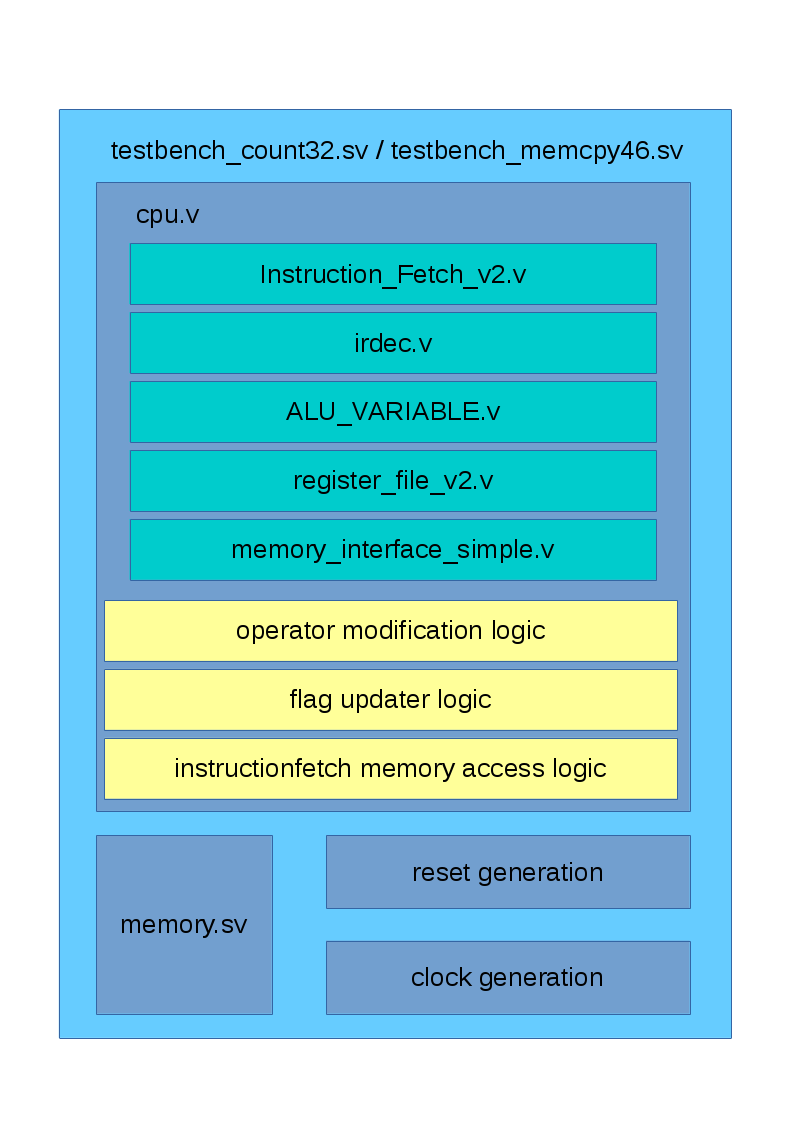
\includegraphics[scale=0.5]{images/rtltestbenchdrawing.png}
\label{fig:rtltestbenchdrawing}
\caption{Structure of the RTL top level testbench}
\end{figure}

\section{Synthesis}
\label{sec:synthesis}

During RTL coding, special attention was given to good coding practice for synthesis, in order to ensure that the synthesized hardware would behave exactly as specified, without any glitches or timing issues. Therefore, each module was separately and iteratively synthesized to make the debugging process more clear and modular. 
The main concern and reason for iterations was the need to avoid using latches in our design, which was solved by carefully assigning all outputs for all input conditions in case or if-else statements. The main reason to avoid the usage of latches is that they are asynchronous storage elements, which would potentially cause timing issues and racing in a fully synchronous design.

Once the final top module was completed, the synthesis iterations were started in order to obtain the fastest hardware possible based on the informations given in the timing report. Starting with a period of 1ns as a constraint, the value was continuously reduced until it was no longer possible to obtain a slack greater than or equal to zero. A negative slack in the timing report means that it is not possible to generate a hardware to the given design that do not violate any timing request with the given period, while a positive or zero slack means that the synthesized hardware could be further optimized.  The value used to synthesize the final hardware was 0.7 ns.

After the synthesis of the final hardware, an analysis of the schematic and the critical path was made in order to compare with the expected from the designed architecture. According to the timing report, the critical path consists of the instruction decoder reading a value from the register file, which is then processed by the ALU and written back to the register file. This path is expected due to the huge amount of combinational logic involved in the process, and the corresponding delay of the critical path is 0.69 ns.

As the guideline was to obtain a processor with the highest possible maximum frequency, there was no concern in optimizing the area or the energy consumption of the final hardware, nor to balance the three performance indicators. As a result, a processor with an area of 22453.12  $\mu m^{2}$ and a power of 6,9367 mW was obtained.
\section{Gate Level Verification}
\label{sec:glverification}

After the synthesis, a gate level simulation is required to check if the behaviour of the final hardware corresponds to the logic simulation performed in the RTL coding stage, as well as to determine the maximum clock frequency under which the processor can run without any timing violations. 

The two timing violations that must be avoided are the setup and hold time violations. A setup violation occurs when a signal does not arrive at a flip-flop with sufficient time, the so called setup time, before the next rising edge of the clock cycle. This means that the circuit is too slow for the critical path. On the other hand, the hold time of a flip-flop is the time that the input signal must remain there after the rising edge of the clock for the output to be safely switched. Therefore, a hold time violation occurs in the shortest paths and means that the circuit is too fast in that region.

With these concepts in mind, a testbench was run for each of the benchmark programs provided for the validation of the final synthesized processor design. Both testbenches were repeatedly run for increasing values of clock speed until any of them presented any timing violations. With this method, the lowest reached clock period under which the processor ran without any errors was 1.26 ns, which corresponds to a maximum frequency of 793 MHz. 
The final value of the clock period is way different than the one used as a timing constraint during the synthesis process, which was 0.7 ns.

\section{Other}
\label{sec:other}

- 
\chapter{Evaluation}
\label{cha:evaluation}

here some stuff on how good this processor is

- what could be better:
  - IT-instruction in fetch
  - better memory controller -lacks time
  - ALU with better solution for multiply (not single cycle)
  - decoder frees fetch earlier
  - 
  
- conclusion:
  - very much work, lack of time
  - trotzdem instruction set working
  


%% Anhang %%%%%%%%%%%%%%%%%%%%%%%%%%%%%%%%%%%%%%%%%%%%%%%%%%%%%%%%%%%%%%%%
%\appendix
\bibliographystyle{plain}
\clearpage
% \nocite{*}
\bibliography{literaturverzeichnis}


\end{document}
